\section{Methodology \& Computer Vision Algorithm}
\label{sec:method}
\subsection{Methodology}
\label{subsec:method}
1. Train a model to recognize faces using the LFW dataset\\
2. Use the trained model to recognize the students in the class.\\
3. Use the Canvas API to fetch the number of students in the class.\\
4. Compare the number of students in the class to the number of students recognized by the model to get a percentage of students in the class.\\
5. Log the percentages and present them in a graph to provide a visual representation of the attendance in the class.\\

The model will be trained using the LFW dataset (Partially). The model will be used to recognize the students in the class. The model will be able to recognize the students in the class and log the time they entered and exited the classroom. The model will also be able to identify the number of students in an image and cross-reference it with Canvas's people table (number of students) to provide a percentage of students in the classroom. The percentages will be logged and presented in a graph to provide a visual representation of the attendance in the class.\\ 
\subsection{Computer Vision Algorithm}
\label{subsec:Computer Vision Algorithm}
Using YOLO \cite{YOLO}, a neural network for object detection, we will train a model to recognize faces. The model will be trained using the LFW dataset. The model will be used to recognize the students in the class. The model will be able to recognize the students in the class and log the time they entered and exited the classroom. The model will also be able to identify the number of students in an image and cross-reference it with Canvas's people table (number of students) to provide a percentage of students in the classroom. The percentages will be logged and presented in a graph to provide a visual representation of the attendance in the class.\\
% Diagram of the system%
\begin{figure}[h]
    \centering
    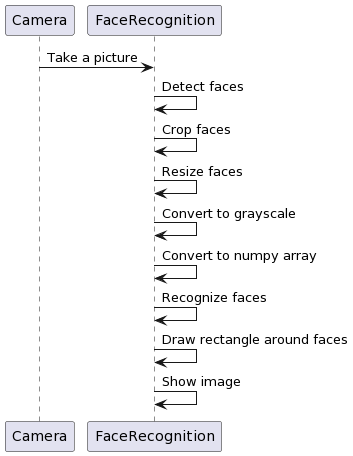
\includegraphics[width=0.5\textwidth]{images/Diagram-1.png}
    \caption{Flowchart of the system}
    \label{fig:flowchart}
\end{figure}






%-------------------------------------------------------------------------
